\documentclass{report}
\usepackage[utf8]{inputenc}
\usepackage{amsmath}
\usepackage{amssymb}
\usepackage{pgfplots}
\usepackage{tikz}
\usepackage{float}
\usepackage[danish]{babel}
\usepackage[margin=1.2in]{geometry}
\usepackage{xcolor}
\usepackage{pdfpages}

\renewcommand{\thesubsection}{\thesection.\alph{subsection}}

\title{Opgave 1, uge 2}
\author{Sebastian Winkelmann}
\date{September 2019}

\begin{document}
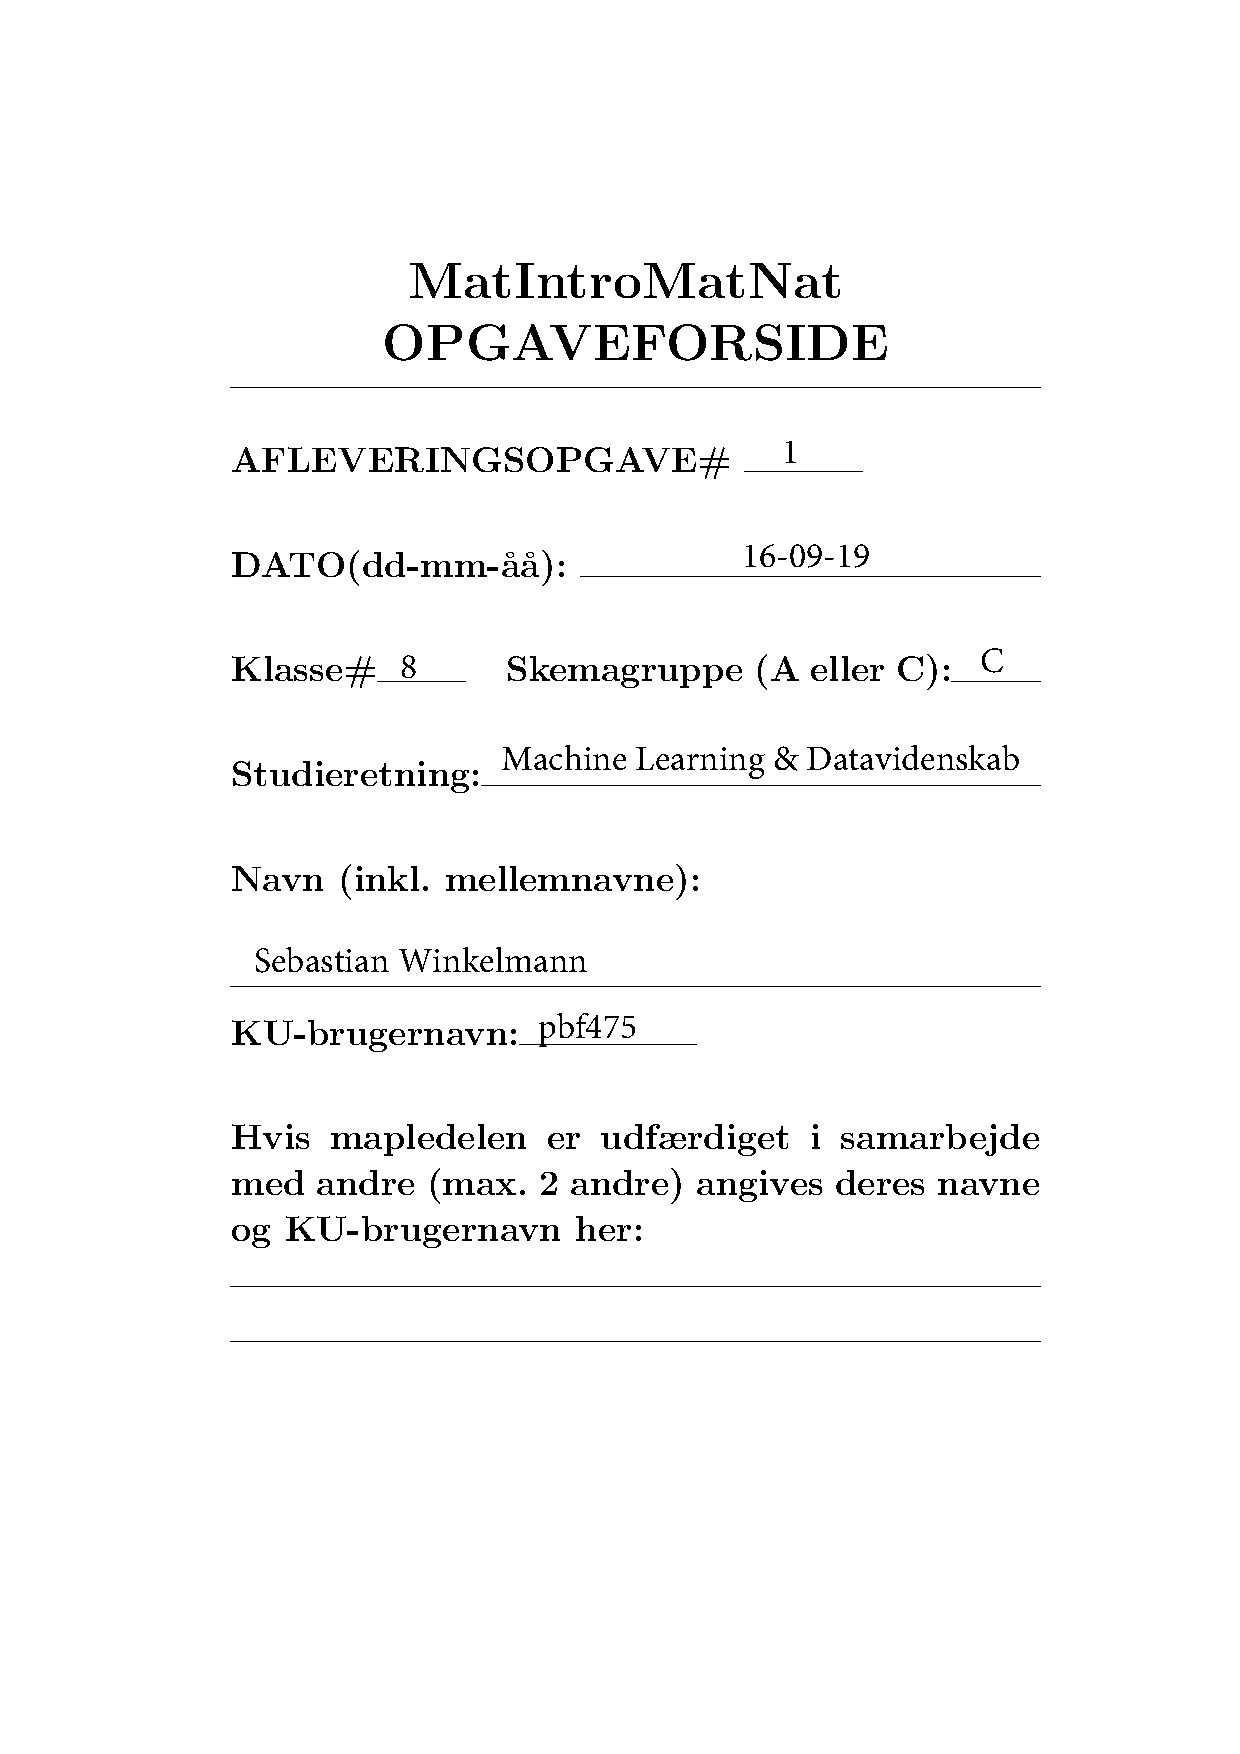
\includepdf{forside.pdf}
\maketitle
\setcounter{chapter}{1}
\section{TLO 3.4.14}
\textit{Find løsningerne til den komplekse ligning}\begin{equation}
    z^2+2(1-i)z+7i=0
\end{equation}
\textbf{Løsning}: Vi kan løse denne som en kompleks andengradsligning ved $$z=\frac{-b\pm\sqrt{b^2-4ac}}{2a}$$
Vi kan altså blot starte med at gange parentesen ud:\begin{align}
    z^2+2(1-i)+7i&=0\\
    z^2+2z-2iz+7i&=0\\
    z^2+(2-2i)z+7i&=0
\end{align}
Vi har den altså på en form som passer ind i $az^2+bz+c=0$. Herved kan vi indsætte
\begin{align}
    z&=\frac{-(2-2i)\pm\sqrt{(2-2i)^2-4\cdot1\cdot7i}}{2\cdot1}\\
    z&=\frac{(-2+2i)\pm\sqrt{(2^2+2^2i^2-2\cdot2\cdot2i)-4\cdot7i}}{2}\\
    z&=\frac{(-2+2i)\pm\sqrt{(4-4-8i)-28i}}{2}\\
    z&=\frac{(-2+2i)\pm\sqrt{-36i}}{2}\\
    z&=\frac{(-2+2i)\pm(6\sqrt{-i})}{2}
\end{align}
Lad os først regne med +:\begin{align}
    z&=\frac{-2+2i+6\sqrt{-i}}{2}\\
    z&=-1+i-3\sqrt{i}
\end{align}
Et tal $-i$ vil have modulus 1 og have argumentet $\theta_{-1}=\frac{3\pi}{2}\land\frac{-\pi}{2}$:\begin{align*}
    -i&=1\cdot e^{-\frac{\pi}{2} i}\\
    &\Updownarrow\\
    \sqrt{-i}&=\sqrt{1\cdot e^{-\frac{\pi}{2} i}}\\
    \sqrt{-i}&=1\cdot\sqrt{e^{-\frac{\pi}{2} i}}\\
    \sqrt{-i}&=1\cdot e^{-\frac{\pi}{4} i}\\
\end{align*}
Vi kan altså konkluderer at det komplekse tal $\sqrt{-i}$ har modulus 1 og argumentet $-\frac{\pi}{4}$. Dette skal ganges med 3, så $$z_2=3\cdot e^{-\frac{\pi}{4}i}$$ Lad os lave det om til normalform:\begin{align*}
    z_2&=3\left(\cos{\frac{\pi}{4}+i\sin{\frac{\pi}{4}}}\right)\\
    z_2&=3\left(\frac{1}{\sqrt{2}}+i\left(-\frac{1}{\sqrt{2}}\right)\right)\\
    z_2&=\frac{3}{\sqrt{2}}-i\frac{3}{\sqrt{2}}
\end{align*}
Vi lægger nu blot de to tal sammen. Først løser vi når leddene adderes\begin{align*}
    z_+&=-1+i+\frac{3}{\sqrt{2}}-i\frac{3}{\sqrt{2}}\\
    z_+&=\left(-1+\frac{3}{\sqrt{2}}\right)+i\left(1-\frac{3}{\sqrt{2}}\right)
\end{align*}
og nu når leddene subtraheres
\begin{align*}
    z_-&=-1+i-\left(\frac{3}{\sqrt{2}}-i\frac{3}{\sqrt{2}}\right)\\
    z_-&=-1+i-\frac{3}{\sqrt{2}}+i\frac{3}{\sqrt{2}}\\
    z_-&=\left(1-\frac{3}{\sqrt{2}}\right)+i\left(1+\frac{3}{\sqrt{2}}\right)
\end{align*}
Vi skal desuden omskrive det til polar form. $z_-$ må ligge i 2. kvadrant ved $\theta_-=\frac{3\pi}{4}$ og $z_+$ må ligge i 4. kvadrant ved $\theta_+-=-\frac{\pi}{2}\lor\frac{7\pi}{4}$. \begin{align*}
    |z_+|&=\sqrt{\left(-1+\frac{3}{\sqrt{2}}\right)^2+\left(1-\frac{3}{\sqrt{2}}\right)^2}\\
    |z_+|&=\sqrt{\left(\frac{3\sqrt{2}-2}{2}\right)^2+\left(2-\frac{3\sqrt{2}}{2}\right)^2}\\
    |z_+|&=\sqrt{\frac{22-12\sqrt{2}}{4}+\frac{22-12\sqrt{2}}{4}}\\
    |z_+|&=\sqrt{\frac{44-24\sqrt{2}}{4}}\\
    |z_+|&=\sqrt{11-6\sqrt{2}}\\
    |z_+|&=\sqrt{\left(3-\sqrt{2}\right)^2}\\
    |z_+|&=3-\sqrt{2}
\end{align*}
Forskellene som er mellem $z_+$ og $z_-$ kan også benyttes her, så vi har at$$|z_-|=\sqrt{2}+3$$
Alt dette kan vi benytte til at omskrive til polær/eksponentialform:\begin{equation}
    z_+=(3-\sqrt{2})e^{i\frac{7\pi}{4}}
\end{equation}og\begin{equation}
    z_-=(\sqrt{2}+3)e^{i\frac{3\pi}{4}}
\end{equation}

Vi kan indtegne dette
\tikzset{every picture/.style={line width=0.75pt}} %set default line width to 0.75pt        
\begin{figure}[H]
    \centering
\begin{tikzpicture}[x=0.75pt,y=0.75pt,yscale=-1,xscale=1]
%uncomment if require: \path (0,491); %set diagram left start at 0, and has height of 491

%Straight Lines [id:da4783664322662121] 
\draw    (135.33,113.47) -- (243,223) ;


%Shape: Square [id:dp9807936632228735] 
\draw   (36,16) -- (243,16) -- (243,223) -- (36,223) -- cycle ;
%Shape: Square [id:dp3818260492162283] 
\draw   (243,16) -- (450,16) -- (450,223) -- (243,223) -- cycle ;
%Shape: Square [id:dp14773382141328928] 
\draw   (36,223) -- (243,223) -- (243,430) -- (36,430) -- cycle ;
%Shape: Square [id:dp44907889391738953] 
\draw   (243,223) -- (450,223) -- (450,430) -- (243,430) -- cycle ;
\draw   (433,215.3) -- (448.88,222.49) -- (433,229.68) ;
\draw   (235.8,33.48) -- (242.89,17.55) -- (250.18,33.39) ;
%Straight Lines [id:da18236117928352857] 
\draw    (36,152.3) -- (46.5,152.25) ;


%Straight Lines [id:da6061528139300535] 
\draw    (36,82.3) -- (46.5,82.25) ;


%Straight Lines [id:da635212026203918] 
\draw    (439,152.3) -- (449.5,152.25) ;


%Straight Lines [id:da5124489441404102] 
\draw    (439,83.3) -- (449.5,83.25) ;


%Straight Lines [id:da5155815069131707] 
\draw    (439,293.3) -- (449.5,293.25) ;


%Straight Lines [id:da7885301992055659] 
\draw    (36,293.3) -- (46.5,293.25) ;


%Straight Lines [id:da48027199901464634] 
\draw    (36,362.3) -- (46.5,362.25) ;


%Straight Lines [id:da6594419456201872] 
\draw    (439,362.3) -- (449.5,362.25) ;


%Straight Lines [id:da5136709527086405] 
\draw    (172.5,420) -- (172.5,430) ;


%Straight Lines [id:da46735268356722237] 
\draw    (102.5,420) -- (102.5,430) ;


%Straight Lines [id:da09560574669828847] 
\draw    (313.5,420) -- (313.5,430) ;


%Straight Lines [id:da20231859118723194] 
\draw    (383.5,420) -- (383.5,430) ;


%Straight Lines [id:da8146600649270341] 
\draw    (313.5,16) -- (313.5,26) ;


%Straight Lines [id:da16039693890225126] 
\draw    (382.5,16) -- (382.5,26) ;


%Straight Lines [id:da3180327378592134] 
\draw    (172.5,16) -- (172.5,26) ;


%Straight Lines [id:da425585075928564] 
\draw    (102.5,16) -- (102.5,26) ;


%Shape: Circle [id:dp07468596263671912] 
\draw  [color={rgb, 255:red, 208; green, 2; blue, 27 }  ,draw opacity=1 ][fill={rgb, 255:red, 208; green, 2; blue, 27 }  ,fill opacity=1 ] (129.64,113.47) .. controls (129.64,110.32) and (132.19,107.77) .. (135.33,107.77) .. controls (138.48,107.77) and (141.02,110.32) .. (141.02,113.47) .. controls (141.02,116.61) and (138.48,119.16) .. (135.33,119.16) .. controls (132.19,119.16) and (129.64,116.61) .. (129.64,113.47) -- cycle ;
%Straight Lines [id:da5654988799977639] 
\draw    (282.88,261.15) -- (243,223) ;


%Shape: Circle [id:dp33602956499899894] 
\draw  [color={rgb, 255:red, 245; green, 166; blue, 35 }  ,draw opacity=1 ][fill={rgb, 255:red, 245; green, 166; blue, 35 }  ,fill opacity=1 ] (277.19,261.15) .. controls (277.19,258.01) and (279.74,255.46) .. (282.88,255.46) .. controls (286.03,255.46) and (288.57,258.01) .. (288.57,261.15) .. controls (288.57,264.29) and (286.03,266.84) .. (282.88,266.84) .. controls (279.74,266.84) and (277.19,264.29) .. (277.19,261.15) -- cycle ;

% Text Node
\draw (472.42,221.75) node  [align=left] {$\displaystyle \mathbb{R} e$};
% Text Node
\draw (243,7) node  [align=left] {$\displaystyle \mathbb{I} m$};
% Text Node
\draw (314.17,441.7) node  [align=left] {$\displaystyle 2$};
% Text Node
\draw (172.17,441.7) node  [align=left] {$\displaystyle -2$};
% Text Node
\draw (102.17,441.7) node  [align=left] {$\displaystyle -4$};
% Text Node
\draw (383.17,441.7) node  [align=left] {$\displaystyle 4$};
% Text Node
\draw (26.17,153.7) node  [align=left] {$\displaystyle 2i$};
% Text Node
\draw (26.17,81.7) node  [align=left] {$\displaystyle 4i$};
% Text Node
\draw (21.17,291.7) node  [align=left] {$\displaystyle -2i$};
% Text Node
\draw (21.17,363.7) node  [align=left] {$\displaystyle -4i$};
\end{tikzpicture}
\caption{De to løsninger indtegnet i den komplekse plan. {\color{red}{$z_-$}} og {\color{yellow}{z_+}}. Håndtegnet i Mathcha}
\end{figure}
\newpage
  
\section{Funktion}
\textit{Betragt funktionen}
\begin{equation}
    f(x)=\frac{3x^2-x-2}{x^2+4x+3},\quad x\in[0,\infty)
\end{equation}
\subsection{Tegn funktionens graf med Maple}
\begin{figure}[H]
    \centering
    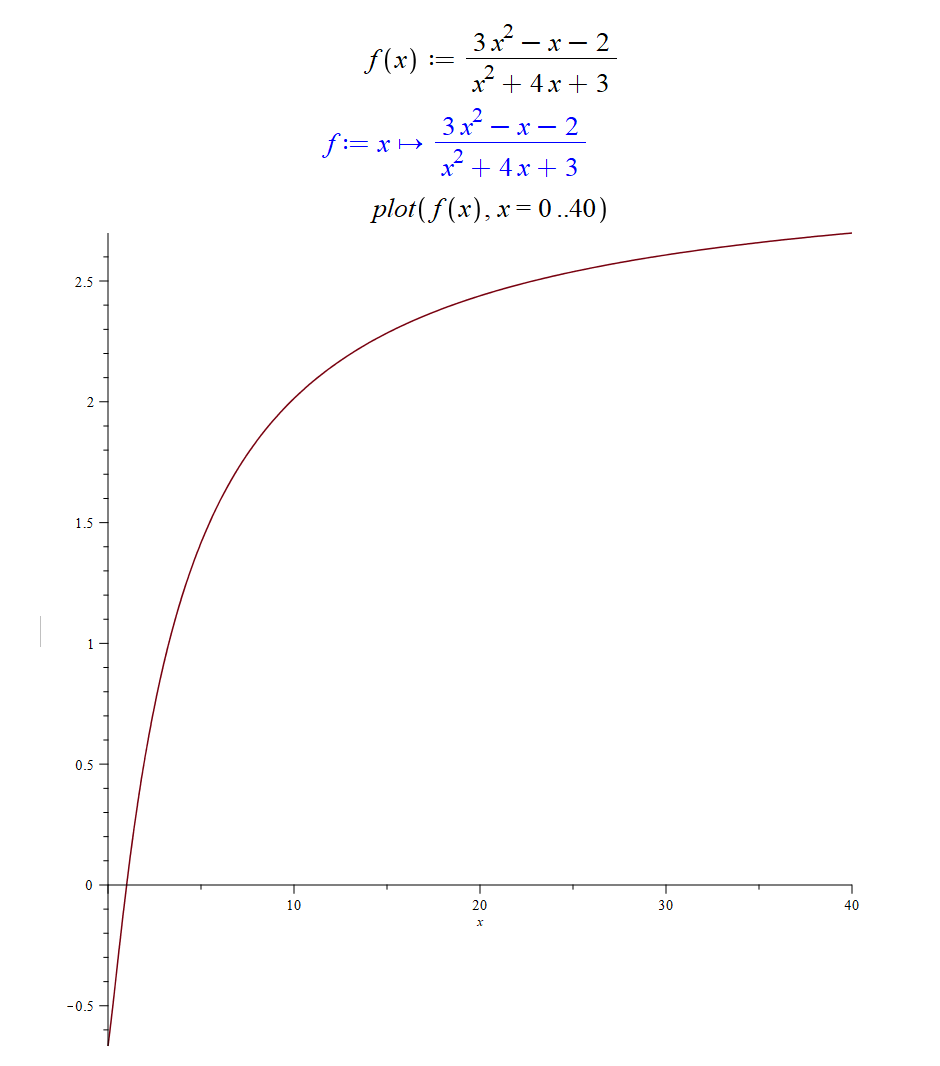
\includegraphics[width=\textwidth]{javaw_5TJhKriajU.png}
\end{figure}
\subsection{Udregn den afledede $f'(x)$ og vis, at den er positiv for alle $x\in[0,\infty)$}
Vi kan differentiere $f$ ved at udnytte kvotientreglen, således at$$\frac{d}{dx}\left(\frac{u}{v}\right)=\frac{v\frac{du}{dx}-u\frac{dv}{dx}}{v^2}$$Vi kan hermed udregne $f'(x)$:
\begin{align*}
    f'(x)&=\frac{(x^2+4x+3)\cdot\frac{d}{dx}(3x^2-x-2)-(3x^2-x-2)\cdot\frac{d}{dx}(x^2+4x+3)}{(x^2+4x+3)^2}\\
    f'(x)&=\frac{(x^2+4x+3)\cdot(6x-1)-(3x^2-x-2)\cdot(2x+4)}{(x^2+4x+3)^2}\\
    f'(x)&=\frac{((6x^3+24x^2+18x)-(x^2+4x+3))-((6x^3-2x^2-4x)+(12x^2-4x-8))}{(x^2+4x+3)^2}\\
    f'(x)&=\frac{6x^3+23x^2+14x-3-(6x^3+10x^2-8x-8)}{(x^2+4x+3)^2}\\
    f'(x)&=\frac{0x^3+13x^2+22x+5}{(x^2+4x+3)^2}\\
    f'(x)&=\frac{13x^2+22x+5}{(x^2+4x+3)^2}
\end{align*}
Det er rimelig tydeligt at nævneren ikke kan blive negativ, i og med der er tale om kvadratet af en størrelse ($n^2\geq0$, $n\in\mathbb{R}$). I kraft af at alle led i tælleren er positive, da må enhver $x_0\geq$ give et positivt tal. Det kan derfor udelukkes at der ved $x\in[0,\infty)$ skulle være et tilfælde hvor $f'(x)<0$. Vi kan desuden udregne dens grænseværdi ved at finde største potens, og dividere igennem med denne eksponent. Den største eksponent er i nævneren, da der efter opløsning af parentes vil stå $x^4$. Vi har altså tilnærmelsesvist
\begin{align*}
    \lim_{x\to\infty}f'(x)&=\lim_{x\to\infty}\frac{13x^2+22x+5}{x^4 + 8 x^3 + 22 x^2 + 24 x + 9}\\\lim_{x\to\infty}f'(x)&=\lim_{x\to\infty}\frac{13x^{-2}+22x^{-3}+5x^{-4}}{x^0 + 8x^{-1} + 22 x^{-2} + 24 x^{-3} + 9x^{-4}}\\\lim_{x\to\infty}f'(x)&=\frac{0}{1}=0
\end{align*}
\subsection{Bestem $\lim_{n\to\infty}f(n)$}\label{subseq:upper}
\begin{align*}
    \lim_{n\to\infty}f(n)&=\lim_{n\to\infty}\frac{3n^2-n-2}{n^2+4n+3}\\
    \text{Igen finder vi den største potens,}&\text{ og dividerer alle led med denne eksponent}\\
    \lim_{n\to\infty}f(n)&=\lim_{n\to\infty}\frac{\frac{3x^2-x-2}{x^2}}{\frac{x^2+4x+3}{x^2}}\\
    \lim_{n\to\infty}f(n)&=\lim_{n\to\infty}\frac{3-\frac{1}{x}-\frac{2}{x^2}}{1+\frac{4}{x}+\frac{3}{x^2}}\\
    \lim_{n\to\infty}f(n)&=\frac{\lim_{n\to\infty}(3-\frac{1}{x}-\frac{2}{x^2})}{\lim_{n\to\infty}(1+\frac{4}{x}+\frac{3}{x^2})}\\
    \text{Da }\lim_{x\to\infty}\frac{1}{x}=0&\text{ simplificeres udtrykket}\\
    \lim_{n\to\infty}f(n)&=\frac{3}{1}\\
    \lim_{n\to\infty}f(n)&=3
\end{align*}
\subsection{Bestem værdimængden for $f$}
Vi har allerede bestemt den øvre grænse for $f$ i sektion \ref{subseq:upper}. Den nedre grænse for funktionen $f$ kan ikke findes som et ekstremumspunkt, da der i forvejen er blevet vist at $f'(x)>0$ når $x\geq0$. Da funktionen i dens definitionsmængde er monoton tiltagende, vil vi således have værdimængden\begin{equation}
    V_f=\left\{y\in\mathbb{R}|-\frac{2}{3}\leq y<3\right\}
\end{equation} da\begin{align*}
    f(0)&=\frac{3x^2-x-2}{x^2+4x+3}\\
    f(0)&=\frac{3(0)^2-0-2}{0^2+4(0)+3}\\
    f(0)&=\frac{0-0-2}{0+0+3}\\
    f(0)&=\frac{-2}{3}
\end{align*}
\subsection{Lad $\epsilon= 0.1$. Bestem en værdi af $N$, som kan anvendes i TL Definisjon 4.3.1, når denne definition benyttes på grænseovergangen i (c). Gentag for $\epsilon=0.01$}
Vi vil undersøge for hvilken værdi $N$ der vil gælde at $$|f(n)-3|<0.1$$ når $n\geq N$.\begin{align*}
    \left|\frac{3n^2-n-2}{n^2+4n+3}-3\right|&<0.1,\quad n\geq0\\&\Downarrow\\n&=126.844
\end{align*}
Vi kan dobbelttjekke resultatet
\begin{align*}
    \frac{3(126.844)^2-126.844-2}{126.844^2+4(126.844)+3}\approxeq2.90000
\end{align*}
Vi vil undersøge for hvilken værdi $N$ der vil gælde at $$|f(n)-3|<0.01$$ når $n\geq N$.\begin{align*}
    \left|\frac{3n^2-n-2}{n^2+4n+3}-3\right|&<0.01,\quad n\geq0\\&\Downarrow\\n&=1296.85
\end{align*}
Vi kan dobbelttjekke resultatet
\begin{align*}
    \frac{3(1296.85)^2-1296.85-2}{1296.85^2+4(1296.85)+3}\approxeq2.99000
\end{align*}
Altså har vi at $N_{\epsilon=0.1}\leq126.844$ og $N_{\epsilon=0.01}\leq1296.85$.
\section{(ii) Banklån}
\textit{Et lån i banken på $L$ kroner forrentes med en årlig rente $r$. Efter det første år skyldes der $L(1 + r)$ på lånet. Tilskriver banken i stedet rente to gange om året, skyldes der efter første halve år $L(1 + r/2)$.}
\subsection{Hvor meget skyldes der i sidstnævnte tilfælde på lånet efter det første år?}
Rentetilskrivning sker ved at sætte parentesen $(1+r/2)$ op i antallet af terminer, $n$. Vi kan altså udregne det ved et år (to årlige terminer):\begin{equation}
    L_2=L(1+r/2)(1+r/2)=L(1+r/2)^2
\end{equation}
Ved $n$ rentetilskrivninger/terminer om året, da vil der efter første år være en gæld på:\begin{equation}
    L_n=L(1+r/n)^n
\end{equation}
Grunden til at man finder gældens størrelse efter $n$ terminer på denne måde er, at når renten er $r$ så skal man gange det originale beløb med $1+r$. Således $$L_n=L\cdot(1+r/n)\cdot(1+r/n)\cdot\! \overbrace{\ldots}^n\cdot(1+r/n)$$
\newpage\subsection{Jo flere årlige rentetilskrivninger jo større er gælden efter første år}
Vi kan lave en funktion i Maple som viser gælden efter $n$ terminer når lånets størrelse $L=100$ og renten $r=10\%$. Plottes i domænet $[0,3]$ da funktionen alligevel flader ud.
\begin{figure}[H]
    \centering
    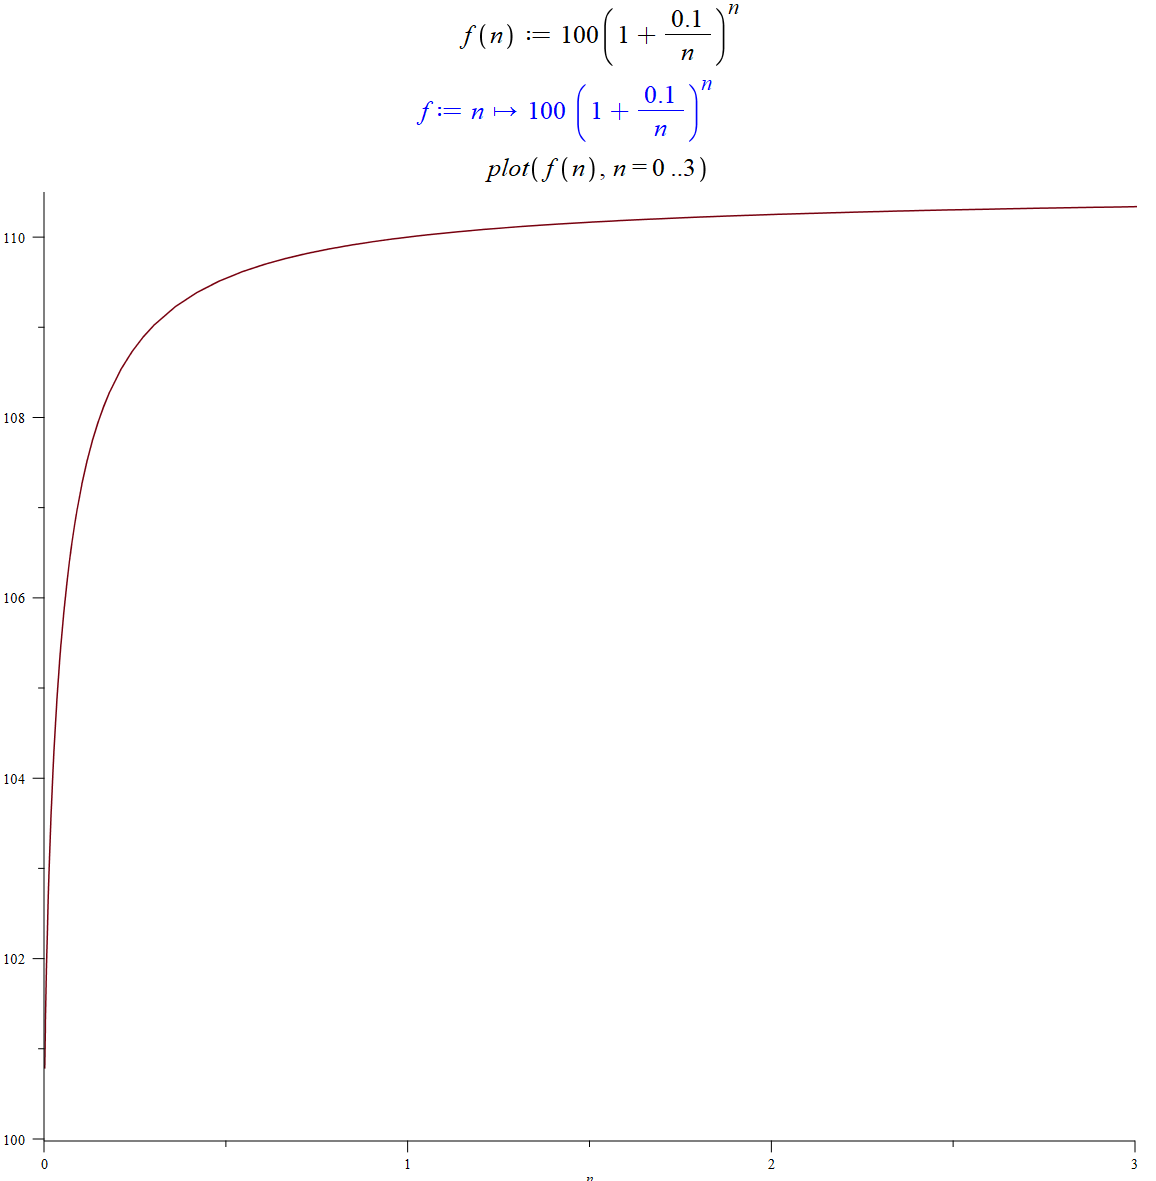
\includegraphics[width=0.9\textwidth]{javaw_WZOXp5TLXq.png}
\end{figure}
Det er altså tydeligt at der tale om en monoton tiltagende funktion som konvergerer. Forskellen i størrelse på gæld er dog minimal. Lad os først se ved $n=1$:\begin{equation}
    L_1=100\left(1+\frac{0.1}{1}\right)^1=100\cdot1.1=110
\end{equation}og nu når $n=2$\begin{equation}
    L_2=100\left(1+\frac{0.1}{2}\right)^2=100\cdot1.05^2=100\cdot1.1025=110.25
\end{equation}Der er altså tale om en meget lille forskel. Ikke desto mindre er der en forskel, og gælden bliver således større jo flere rentetilskrivninger der er årligt.

\subsection{Argumenter for, at gælden efter første år enten divergerer mod uendelig eller konvergerer, når antallet af rentetilskrivninger n går mod uendelig (kontinuert rentetilskrivning)}
Rentetilskrivningsfunktionen $R(n)=(1+r/n)^n$ vil konvergere. Det giver desuden fint logisk mening at når renten bliver splittet op i mindre og mindre dele, så vil det blive meget småt. Det er desuden definitionen af eksponentialfunktionen:$$\lim_{x\to x}\left(1+\frac{1}{x}\right)^x=e$$så der må tilsvarende være en grænseværdi her. Vi kan vise dette ved at tage en grænseværdi:\begin{align*}
    \lim_{n\to\infty}f(n)&=\lim_{n\to\infty}L(1+r/n)^n\\
    &=L\lim_{n\to\infty}\exp{\left(\log{((1+r/n)^n)}\right)}\\
    &=L\lim_{n\to\infty}\exp{\left(n\log{(1+r/n)}\right)}\\
    &=L\exp{\lim_{n\to\infty}\left(n\log{(1+r/n)}\right)}\\
    \text{Vi kan benytte}&\text{ l'Hôpitals regel}\\
    &=L\exp{\left(\lim_{n\to\infty}\left(\frac{\log{(1+r/n)}}{1/n}\right)\right)}\\
    \text{Da }\log{1}=0&\text{ giver udtrykket }\frac{0}{0}.\\
    &=L\exp{\left(\lim_{n\to\infty}\left(\frac{r\cdot n}{n+r}\right)\right)}\\
    &=L\exp{\left(r\lim_{n\to\infty}\left(\frac{n}{n+r}\right)\right)}\\
    \text{Dividerer}&\text{ igennem med }n\\
    &=L\exp{\left(r\lim_{n\to\infty}\left(\frac{n/n}{n/n+r/n}\right)\right)}\\
    &=L\exp{\left(r\lim_{n\to\infty}\left(\frac{1}{1+r/n}\right)\right)}\\
    &=L\exp{\left(r\left(\frac{1}{1+0}\right)\right)}\\
    &=L\exp{(r\cdot1)}\\
    &=Le^{r}
\end{align*}
\end{document}